\documentclass[aspectratio=1610]{beamer}
\usefonttheme{professionalfonts}
\usetheme{metropolis}
\setbeamertemplate{bibliography item}{\insertbiblabel}
\usepackage{polyglossia}
\setmainlanguage{english}
\usepackage{amsmath}
\usepackage{amssymb}
\usepackage{mathtools}
\usepackage{graphicx}
\usepackage[version=4]{mhchem}
\usepackage[
  math-style=ISO,
  bold-style=ISO,
  sans-style=italic,
  nabla=upright,
]{unicode-math}
\setmathfont{Latin Modern Math}
\usepackage{blindtext}
\usepackage{fontspec}
\title{}
\subtitle{}
\date{\today}
\author{Steven Becker}
\usepackage{siunitx}
\AtBeginDocument{
\sisetup{
math-rm=\mathrm,
math-micro=μ,
}
}
\usepackage{framed}
\usepackage{biblatex}
\addbibresource{lit.bib}
\usepackage{booktabs}

\begin{document}

\frame{\maketitle}



\begin{frame}{ Überblick }
  \begin{itemize}
    \setlength\itemsep{1.2em}
      \item{ Situation in Deutschland }
      \item{ Weg zur Stillegung }
      \item{ Der Rückbau }
      \item{ Kosten }
  \end{itemize}
\end{frame}



\begin{frame}{ Situation in Deutschland }
  \begin{figure}
     \centering
     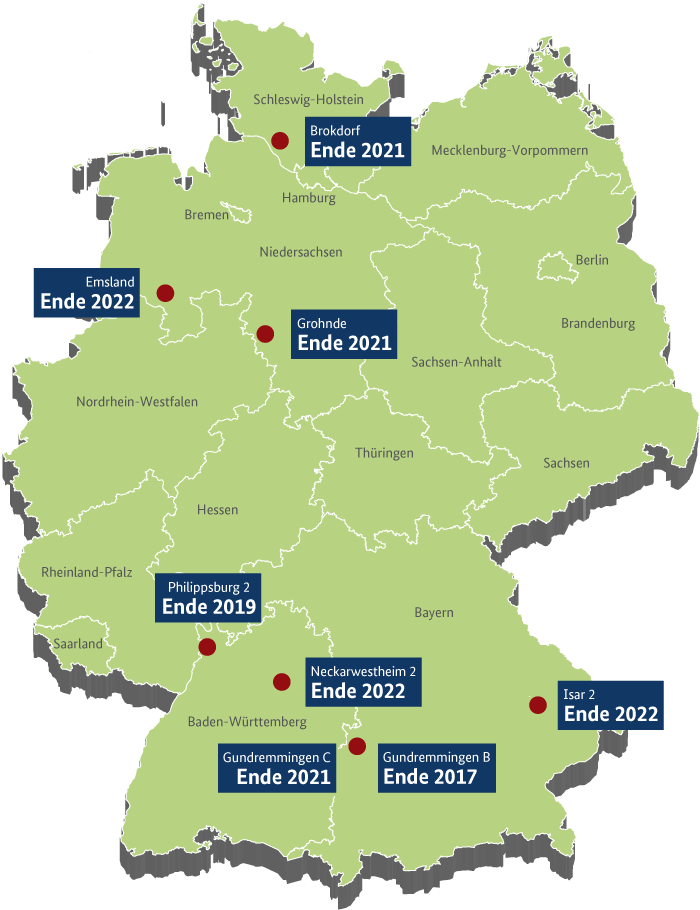
\includegraphics[width=0.4\textwidth]{./bilder/akw_abschaltung_karte.png}
     \caption{ Auflistung der Abschaltungsjahre von deutschen AKWs \cite{ karte_abschaltungen }. }
     \label{ fig: karte_abschaltungen }
   \end{figure}
\end{frame}



\begin{frame}{ Weg zu Stillegung }
  \begin{itemize}
    \setlength\itemsep{1.2em}
      \item{ Stillegungen müssen beantragt werden}
      \item{ Länder sind dafür zuständig}
      \item{ Unterliegt dem Atomrecht}
  \end{itemize}
\end{frame}



\begin{frame}{ Weg zur Stillegung }
  \begin{figure}
     \centering
     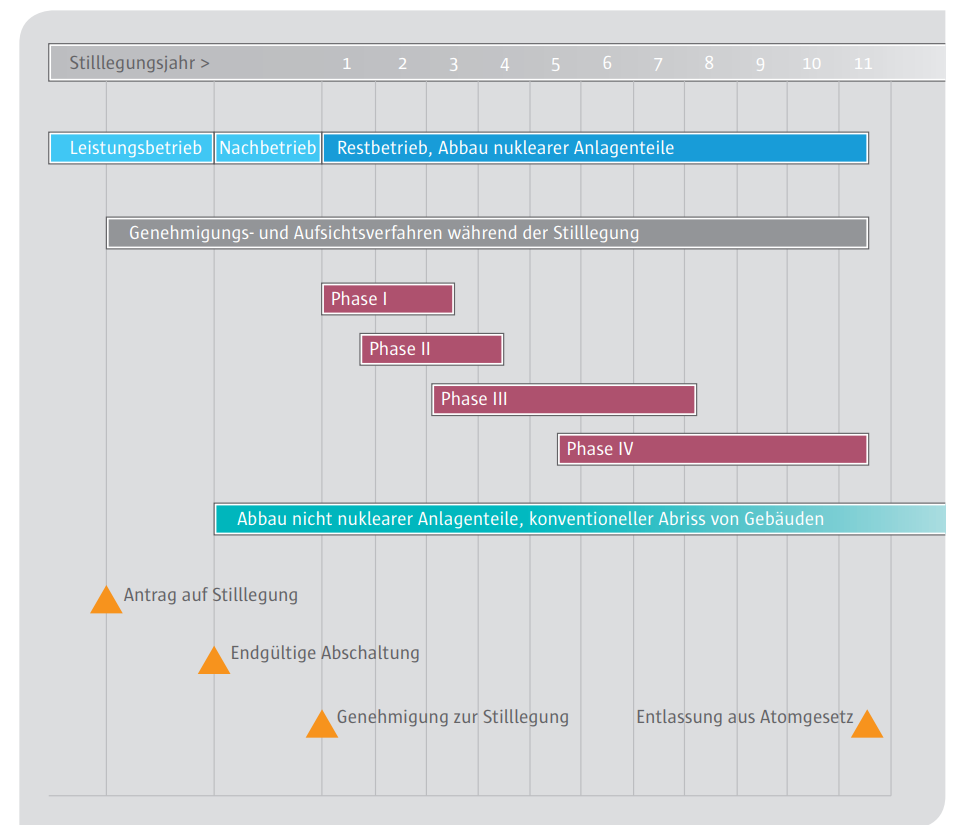
\includegraphics[width=0.6\textwidth]{./bilder/stillegungs_zeit_2_kernfragen.PNG}
     \caption{ Zeitlicher Verlauf einer Stillegung \cite{ stilllegung_grs }. }
     \label{ fig: stillegung }
   \end{figure}
\end{frame}



\begin{frame}[allowframebreaks]
  \nocite{*}
  \printbibliography
\end{frame}

\end{document}
